\chapter{Измерение, матрицы плотности и энтропия}

Эксперимент с двумя щелями содержит проблему измерения в её наименьшей полезной форме. Когда две альтернативы остаются когерентными, их амплитуды интерферируют. Когда другая система получает запись о том, какая альтернатива реализовалась, объект и регистратор запутываются, и интерференция изменяется. Прежде чем вводить след, матрицу плотности и энтропию --- язык, необходимый для количественного описания запутанности, мы сделаем этот механизм точным.

\section{Восстановление эксперимента с двумя щелями}

Рассмотрим дискретную модель с источником в узле \(0\), двумя отверстиями \(A\) и \(B\) и экраном, возможные узлы попадания на котором представлены ортонормированными состояниями \(\{|m\rangle\}\). Частица может быть электроном, фотоном или любым другим квантовым объектом. Будем называть её электроном и пренебрежём её собственным спином, так что обсуждаемой степенью свободы остаётся только положение. Остальная часть преграды закрыта: электрон, достигающий любого узла, кроме \(A\) или \(B\), отражается.

Структурный принцип здесь — линейность. Если два состояния эволюционируют как
\begin{equation}
|A\rangle\longrightarrow |A'\rangle,
\qquad
|B\rangle\longrightarrow |B'\rangle,
\end{equation}
то любая суперпозиция эволюционирует с теми же коэффициентами:
\begin{equation}
\alpha|A\rangle+\beta|B\rangle
\longrightarrow
\alpha|A'\rangle+\beta|B'\rangle.
\end{equation}

В симметричной конфигурации источник подаёт на оба отверстия одинаковую амплитуду. Опуская общий нормировочный множитель, как на доске,
\begin{equation}
|0\rangle\longrightarrow |A\rangle+|B\rangle.
\end{equation}
Нормированное состояние имело бы вид \((|A\rangle+|B\rangle)/\sqrt{2}\); опущенный множитель не играет никакой роли в рассуждении об интерференции.

Теперь рассмотрим каждый маршрут по отдельности. Распространение от отверстий к экрану имеет вид
\begin{align}
|A\rangle &\longrightarrow \sum_m \psi_m|m\rangle, \\
|B\rangle &\longrightarrow \sum_m \phi_m|m\rangle.
\end{align}
Комплексное число \(\psi_m\) есть амплитуда прихода в узел экрана \(m\) при старте из \(A\), а \(\phi_m\) — соответствующая амплитуда при старте из \(B\).

\begin{figure}[htbp]
\centering
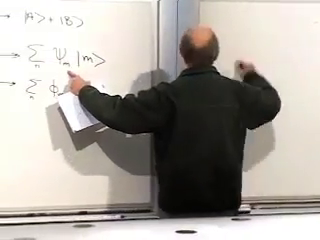
\includegraphics[width=0.68\textwidth]{lecture_07_figure_02.png}
\caption{Разложения по базису экрана для отдельных маршрутов через \(A\) и \(B\).}
\lectureframe{00:05:39}
\end{figure}

Если \(B\) закрыто, вероятность попасть в \(m\) равна
\begin{equation}
P_A(m)=|\psi_m|^2.
\end{equation}
Если закрыто \(A\),
\begin{equation}
P_B(m)=|\phi_m|^2.
\end{equation}
Классическая вероятность подсказывала бы сложить эти два результата, когда доступны оба отверстия. Квантовая механика вместо этого сначала складывает амплитуды:
\begin{equation}
|A\rangle+|B\rangle
\longrightarrow
\sum_m(\psi_m+\phi_m)|m\rangle.
\end{equation}
В фиксированном узле экрана
\begin{align}
P(m)
&=|\psi_m+\phi_m|^2 \\
&=|\psi_m|^2+|\phi_m|^2
  +\psi_m^*\phi_m+\phi_m^*\psi_m.
\end{align}

\begin{figure}[htbp]
\centering
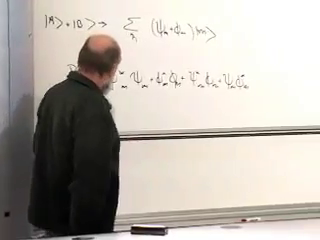
\includegraphics[width=0.70\textwidth]{lecture_07_figure_03.png}
\caption{Четырёхчленная вероятность на экране. Последние два слагаемых — интерференционные члены.}
\lectureframe{00:09:21}
\end{figure}

В точке симметрии \(\psi_m=\phi_m\), и две альтернативы усиливают друг друга. В точке, где их фазы различаются на \(\pi\), \(\psi_m=-\phi_m\), вероятность обращается в нуль. Каждым маршрутом по отдельности этой точки можно достичь, однако открытие обоих маршрутов может помешать электрону попасть туда. Теперь вопрос неизбежен: что меняется, когда нечто регистрирует, какое отверстие было использовано?

\section{Детектор становится запутанным}

Введём вспомогательную двухуровневую систему с состояниями \(|u\rangle\) и \(|d\rangle\). В этой модели это не спин электрона; это минимальный внешний прибор. Изначально детектор не сработал:
\begin{equation}
|0,d\rangle.
\end{equation}
Организуем взаимодействие так, чтобы прохождение через \(A\) переворачивало спин детектора, тогда как прохождение через \(B\) оставляло его без изменения:
\begin{equation}
|0,d\rangle
\longrightarrow
|A,u\rangle+|B,d\rangle.
\end{equation}
После того как электрон проходит отверстия, он больше не взаимодействует со вспомогательным спином. Поэтому две ветви далее распространяются как
\begin{align}
|A,u\rangle &\longrightarrow \sum_m\psi_m|m,u\rangle, \\
|B,d\rangle &\longrightarrow \sum_m\phi_m|m,d\rangle,
\end{align}
а конечное состояние имеет вид
\begin{equation}
|\Psi\rangle
=\sum_m\left(\psi_m|m,u\rangle+\phi_m|m,d\rangle\right).
\end{equation}
Теперь маршрут и запись детектора запутаны. Считывание детектора показало бы, какое отверстие было использовано.

\begin{classroomqa}
\lecturetimestamp{00:13:24}
\audiencequestion{Произошёл ли уже коллапс волнового пакета, когда спин переворачивается?}
\lecturerresponse{Если рассматривать только электрон, можно использовать язык коллапса: маршрутные альтернативы больше не интерферируют. Однако для полной системы электрон--детектор ни одна ветвь не отброшена. Состояние по-прежнему равно \(|A,u\rangle+|B,d\rangle\). Учёт прибора заменяет утверждение \emph{электрон коллапсировал} точным утверждением о том, что установилась запутанность системы--аппарата.}
\end{classroomqa}

Вспомогательный спин — лишь удобный указатель. Ту же роль могут играть сработавший или несработавший прибор, испущенный или отсутствующий фотон либо любая другая пара различимых записей.

\begin{classroomqa}
\lecturetimestamp{00:15:17}
\audiencequestion{Всегда ли само прохождение через металлическую пластину оставляет запись о маршруте?}
\lecturerresponse{Не обязательно. Существенно то, оставляет ли взаимодействие пластину в различимых конечных состояниях. Если у пластины есть энергетическая щель и электрону не хватает энергии, чтобы её возбудить, никакого долговременного внутреннего следа может не остаться. Самого взаимодействия недостаточно; две альтернативы должны скоррелироваться с различимыми записями.}
\end{classroomqa}

\begin{classroomqa}
\lecturetimestamp{00:16:29}
\audiencequestion{Может ли отдача пластины показать, прошёл ли электрон через верхнее или нижнее отверстие?}
\lecturerresponse{Только если противоположно направленные импульсные толчки создают достаточно различимые состояния пластины. У хорошо локализованной пластины волновая функция по импульсу и без того широка. Малые сдвиги вверх и вниз могут почти полностью перекрываться, так что состояния отдачи не ортогональны и не дают однозначной записи маршрута. Здесь интерференцию защищает принцип неопределённости.}
\end{classroomqa}

Частичная запись возможна. Если детектор получает лишь слабый толчок, два конечных состояния записи не обязаны быть ортогональными. Тогда интерференция не исчезает, а лишь ослабляется. Для формального вычисления мы сначала возьмём предельный случай полного измерения:
\begin{equation}
\langle u|d\rangle=0.
\end{equation}

\section{Расчёт с проектором}

Теперь вычислим вероятность того, что электрон приходит в фиксированный узел экрана \(m\), не спрашивая о результате детектора. В объединённом пространстве Гильберта свойство \emph{электрон в узле \(m\)} представляет собой двумерное подпространство, натянутое на
\begin{equation}
|m,u\rangle,\qquad |m,d\rangle.
\end{equation}
Соответствующий проектор равен
\begin{equation}
\Pi_m
=|m,u\rangle\langle m,u|
 +|m,d\rangle\langle m,d|.
\end{equation}

\begin{figure}[htbp]
\centering
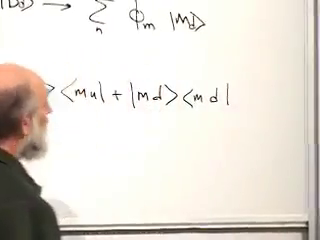
\includegraphics[width=0.66\textwidth]{lecture_07_figure_04.png}
\caption{Проектор на фиксированное положение на экране, просуммированный по двум ортогональным записям детектора.}
\lectureframe{00:22:04}
\end{figure}

Постулат вероятности даёт
\begin{equation}
P(m)=\langle\Psi|\Pi_m|\Psi\rangle.
\end{equation}
Расписывая суммы, получаем
\begin{align}
P(m)
&=
\sum_{n,n'}
\left(\psi_n^*\langle n,u|+\phi_n^*\langle n,d|\right)
\notag\\
&\quad\times\Pi_m
\notag\\
&\quad\times
\left(\psi_{n'}|n',u\rangle+\phi_{n'}|n',d\rangle\right).
\end{align}
Скалярные произведения по координатным состояниям требуют \(n=m=n'\). Скалярные произведения по состояниям детектора затем определяют, какие члены остаются:
\begin{align}
\langle u|u\rangle&=1,
&
\langle d|d\rangle&=1,
&
\langle u|d\rangle&=\langle d|u\rangle=0.
\end{align}
Следовательно,
\begin{equation}
P(m)=|\psi_m|^2+|\phi_m|^2.
\end{equation}

Перекрёстные члены не были устранены по произвольному предписанию. Они обращаются в нуль потому, что две маршрутные амплитуды теперь умножают ортогональные векторы расширенного пространства состояний. Чтобы интерферировать, альтернативы должны совпадать не только в конечной точке на экране, но и по каждой степени свободы, которая несёт запись.

\section{Что считается измерением?}

Простая модель со спином даёт общее правило: измерение происходит тогда, когда взаимодействие устанавливает корреляцию между альтернативами системы и различимыми состояниями прибора. Следующие варианты проверяют это правило.

\begin{classroomqa}
\lecturetimestamp{00:26:53}
\audiencequestion{Что если спин расположен симметрично и переворачивается при прохождении через любое из отверстий?}
\lecturerresponse{Тогда обе ветви несут одну и ту же запись, \(|A,u\rangle+|B,u\rangle=(|A\rangle+|B\rangle)\otimes|u\rangle\). Состояние детектора выносится общим множителем и не раскрывает никакой информации о маршруте, так что интерференционная картина сохраняется.}
\end{classroomqa}

\begin{figure}[htbp]
\centering
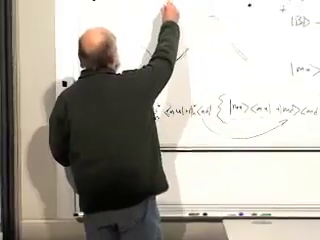
\includegraphics[width=0.68\textwidth]{lecture_07_figure_05.png}
\caption{Вариант на доске, в котором симметрично расположенный детектор одинаково реагирует на оба маршрута.}
\lectureframe{00:27:14}
\end{figure}

\begin{figure}[htbp]
\centering
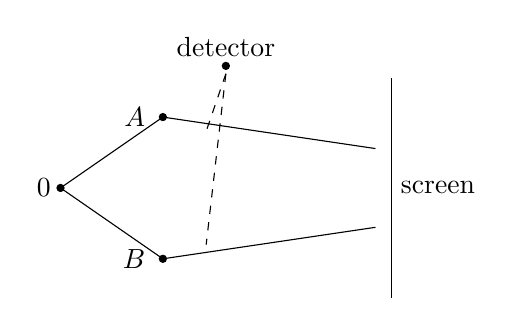
\begin{tikzpicture}[scale=1.0]
\fill (-2,0) circle (1.5pt);
\node[left] at (-2,0) {$0$};
\fill (-0.7,0.9) circle (1.5pt);
\node[left] at (-0.8,0.9) {$A$};
\fill (-0.7,-0.9) circle (1.5pt);
\node[left] at (-0.8,-0.9) {$B$};
\draw (-2,0) -- (-0.7,0.9);
\draw (-2,0) -- (-0.7,-0.9);
\draw (-0.7,0.9) -- (2.0,0.5);
\draw (-0.7,-0.9) -- (2.0,-0.5);
\draw (2.2,-1.4) -- (2.2,1.4);
\node[right] at (2.2,0) {screen};
\fill (0.1,1.55) circle (1.5pt);
\node[above] at (0.1,1.55) {detector};
\draw[dashed] (0.1,1.45) -- (-0.15,0.72);
\draw[dashed] (0.1,1.45) -- (-0.15,-0.72);
\end{tikzpicture}
\caption{Аккуратная реконструкция симметричного расположения детектора: оба маршрута приводят к одному и тому же состоянию детектора.}
\end{figure}

\begin{classroomqa}
\lecturetimestamp{00:27:55}
\audiencequestion{Должен ли кто-то действительно считывать вспомогательный спин, прежде чем интерференция исчезнет?}
\lecturerresponse{Нет. Электрон уже скоррелировал свой маршрут со спином. Можно сбросить детектор, повторять эксперимент, пропуская электроны по одному, и смотреть только на распределение попаданий по экрану. Полосы отсутствуют, даже если никто не считывает спин; значение имеет физическая запись, а не человеческое осознание её.}
\end{classroomqa}

\begin{classroomqa}
\lecturetimestamp{00:29:36}
\audiencequestion{Разрушила бы интерференцию достаточно лёгкая пластина, испытывающая отдачу?}
\lecturerresponse{Да, если отдача переводит пластину в ортогональные импульсные состояния для двух маршрутов. Если сдвинутые волновые пакеты всё ещё перекрываются, разрушение лишь частично. Критерием служит не масса сама по себе, а различимость конечных состояний пластины.}
\end{classroomqa}

Излучение даёт ещё один несовершенный регистратор. Ускоренная заряженная частица может испустить фотон. Излучение, испущенное вблизи \(A\), не обязано совпадать по состоянию с излучением, испущенным вблизи \(B\), так что электромагнитное поле может сохранить информацию о маршруте. Для электрона, отклоняемого медленно, вероятность испускания может быть малой; в лекции для наглядности используется оценка порядка одного случая из ста. Более сильное ускорение делает излучение и, следовательно, потерю контраста более вероятными. Важный пункт качественный: даже ненаблюдаемый фотон может унести когерентность.

\begin{classroomqa}
\lecturetimestamp{00:32:00}
\audiencequestion{Как в реальном эксперименте с несовершенным контрастом определяют вероятность интерференции?}
\lecturerresponse{Эксперимент повторяют много раз и оценивают распределение на экране по относительным частотам. Конечный объём выборки и записи, оставленные окружением, приводят к остаточным отсчётам в областях, которые номинально должны быть тёмными. По мере увеличения числа испытаний оценённое распределение вероятностей улучшается, тогда как декогерирующие процессы уменьшают физический контраст полос.}
\end{classroomqa}

\begin{classroomqa}
\lecturetimestamp{00:33:13}
\audiencequestion{Уничтожает ли всякая возможность определить путь всю интерференцию?}
\lecturerresponse{Полная различимость уничтожает её полностью. Частичная информация приводит к частичной потере. Детектор, который поворачивается лишь немного, оставляет два неортогональных состояния записи, так что при считывании детектора один путь становится более вероятным, чем другой, но не определённым наверняка; соответственно, полосы размываются, а не стираются.}
\end{classroomqa}

Пусть \(|E_A\rangle\) и \(|E_B\rangle\) обозначают произвольные состояния записи. Совместное состояние на экране можно записать как
\begin{equation}
|\Psi\rangle
=\sum_m\left(
\psi_m|m\rangle|E_A\rangle
+\phi_m|m\rangle|E_B\rangle
\right).
\end{equation}
Если пренебречь системой записи, получаем
\begin{align}
P(m)
&=|\psi_m|^2+|\phi_m|^2 \\
&\quad
+\psi_m^*\phi_m\langle E_A|E_B\rangle
+\phi_m^*\psi_m\langle E_B|E_A\rangle.
\end{align}
Следовательно, перекрытие \(\langle E_A|E_B\rangle\) есть фактор когерентности. Идентичные записи сохраняют полную интерференцию; ортогональные записи устраняют её; промежуточное перекрытие даёт промежуточную видимость.

\begin{classroomqa}
\lecturetimestamp{00:34:12}
\audiencequestion{Если фотоны испускаются лишь изредка, что произойдёт, если оставить только события с испусканием фотона?}
\lecturerresponse{В этом отобранном подансамбле интерференция, как правило, хуже, потому что фотон несёт информацию о пути. Потеря не обязана быть полной: волновые пакеты фотонов, испущенных в двух отверстиях, сами могут перекрываться, так что даже излучательные записи могут не быть идеально ортогональными.}
\end{classroomqa}

Воздействие окружающей среды переносит этот механизм на макроскопический уровень. Молекулы воздуха, фоновые фотоны и окружающее вещество непрерывно приобретают записи о макроскопических положениях. Человек или Луна не остаются заметно размазанными по когерентной суперпозиции положений: масса замедляет свободное расплывание, а непрерывная запутанность с окружением подавляет наблюдаемую интерференцию между макроскопически разделёнными альтернативами.

\begin{classroomqa}
\lecturetimestamp{00:36:02}
\audiencequestion{Является ли это уже теорией измерения, а не просто ещё одним употреблением выражения \emph{коллапс волнового пакета}?}
\lecturerresponse{Это и есть механизм в намеренно точном примере. В описании, включающем только электрон, коллапс означает отбрасывание внедиагональных членов \(\psi^*\phi\). В составном описании никакого специального удаления не требуется: запутанность с ортогональными состояниями прибора делает эти члены недоступными для измерений, проводимых только над электроном. Более сложные примеры следует сводить к этой структуре.}
\end{classroomqa}

\begin{classroomqa}
\lecturetimestamp{00:38:04}
\audiencequestion{Изменит ли гравитационное поле, искривляющее путь, естественным образом рассуждение об излучении или правило интерференции?}
\lecturerresponse{Подробности излучения могут измениться, и квантовая механика не приписывает единственную чёткую траекторию до измерения пути. Общий вывод не меняется: интерференцию подавляет только такая степень свободы, которая сохраняет различимую информацию о пути. Пока не указан конкретный прибор, более подробный ответ не имеет смысла.}
\end{classroomqa}

\begin{classroomqa}
\lecturetimestamp{00:39:44}
\audiencequestion{Отличается ли эта интерференция от интерференции классических электромагнитных волн?}
\lecturerresponse{Для многих фотонов наблюдаемая картина согласуется с обычной волновой интерференцией электромагнитного поля. Одночастичный эксперимент показывает более глубокое квантовое утверждение: фотоны и электроны приходят как отдельные события, тогда как интерферируют их квантовые амплитуды. Для электронов соответствующая волна — это электронная волновая функция, а не электромагнитная волна.}
\end{classroomqa}

\begin{classroomqa}
\lecturetimestamp{00:40:45}
\audiencequestion{Что происходит с частями начальной волны, направленными между \(A\) и \(B\)?}
\lecturerresponse{В этой намеренно дискретной модели остальная часть преграды закрыта. Эти части отражаются и не вносят вклада в прошедшую к экрану амплитуду. Модель выделяет две прошедшие альтернативы, не утверждая, что у реального пучка есть только две компоненты импульса.}
\end{classroomqa}

\section{Кот, экран и подвижная граница}

Та же математика применима к коту Schr\"odinger. Пусть у ружья состояния \(|U\rangle\) и \(|F\rangle\) соответствуют отсутствию выстрела и выстрелу, а у кота состояния \(|L\rangle\) и \(|D\rangle\) — жизни и смерти. Начиная с живого кота и ружья без выстрела, взаимодействие может дать
\begin{equation}
|\Psi_{\mathrm{cat}}\rangle
=\alpha|L,U\rangle+\beta|D,F\rangle.
\end{equation}
Сам по себе кот не находится в когерентном состоянии \(\alpha|L\rangle+\beta|D\rangle\). Он запутан с ружьём, которое зарегистрировало альтернативу. Взглянув на ружьё, можно узнать, в какой ветви находится кот, а ортогональные записи ружья устраняют в подсистеме кота обычную интерференцию между живым--мёртвым состояниями.

\begin{classroomqa}
\lecturetimestamp{00:41:18}
\audiencequestion{Находится ли сам кот в суперпозиции живого и мёртвого?}
\lecturerresponse{Не в простом изолированном смысле. Составная система кот--ружьё находится в суперпозиции коррелированных альтернатив: живой при отсутствии выстрела и мёртвый после выстрела. Подсистема кота запутана с ружьём, несущим запись, точно так же, как путь электрона запутан со вспомогательным спином.}
\end{classroomqa}

Конечный экран тоже нужно рассматривать как прибор. Электрон, приходящий в \(m\), может почернить фотозерно, заставить сцинтиллятор испустить фотон или переключить один детектор в ряду локальных двухсостояний устройств. Метка становится коррелированной с положением прихода.

\begin{classroomqa}
\lecturetimestamp{00:43:38}
\audiencequestion{Почему мы можем говорить о вероятностях на конечном экране, а не всё время оперировать только векторами состояния?}
\lecturerresponse{Постулат вероятности приписывает \(\langle\Pi_m\rangle\) свойству \emph{прибытие в \(m\)}. Чтобы завершить физический эксперимент, экран затем оставляет запись положения. Проектор задаёт вероятность; почернение, сцинтилляция или переключение локального детектора реализуют то измерение, статистика которого и собирается.}
\end{classroomqa}

\begin{classroomqa}
\lecturetimestamp{00:45:00}
\audiencequestion{Почему обсуждается измерение на экране, но не вероятность прохождения через \(A\) или \(B\)?}
\lecturerresponse{Приписывать и проверять вероятности путей можно только установив регистратор пути. Без такой записи альтернативы остаются когерентными, и их нужно складывать как амплитуды. Для экрана предполагается прибор, чувствительный к положению. Различие определяется не привилегированным моментом времени, а тем, организовано ли соответствующее измерительное взаимодействие.}
\end{classroomqa}

Границу между системой и прибором можно сдвигать. Включим наблюдателя с состояниями записи \(|O_u\rangle\) и \(|O_d\rangle\); тогда
\begin{equation}
|A,u\rangle+|B,d\rangle
\longrightarrow
|A,u,O_u\rangle+|B,d,O_d\rangle.
\end{equation}
С первым, в свою очередь, может коррелироваться другой наблюдатель. Дым в коробке с котом, ружьё, кот, Schr\"odinger и Вигнер — всё это можно включить в одну более длинную цепочку запутанности. Где бы ни проводили границу, корреляции должны оставаться согласованными: если Вигнер позже спросит Schr\"odinger, что тот видел, их записи совпадут.

\begin{classroomqa}
\lecturetimestamp{00:47:24}
\audiencequestion{Где именно должна оканчиваться система и начинаться измеряющий наблюдатель?}
\lecturerresponse{Квантовая механика не выбирает единственную удобную границу. Можно применить коллапс к описанию только электрона, включить детектор и применить коллапс к более широкому описанию, или включить наблюдателя и снова расширить запутанное состояние. Физическое требование состоит в согласованности всех доступных вероятностей и записей, а не в единственной границе, продиктованной способом учёта.}
\end{classroomqa}

\begin{classroomqa}
\lecturetimestamp{00:49:47}
\audiencequestion{Входит ли сюда принцип неопределённости потому, что измерение пути возмущает событие?}
\lecturerresponse{Да. Пример с отдачей делает эту связь явной: локализация пластины влечёт неопределённость импульса, которая может не дать малым зависящим от пути толчкам стать различимыми. В более общем виде квантовое измерение не завершено, пока запутанность система--прибор не изменила состояние, а это изменение может повлиять на последующую интерференцию.}
\end{classroomqa}

Это резко контрастирует с классическим идеалом. В классике воображают, что измерение можно сделать сколь угодно щадящим и извлечь информацию при пренебрежимо малом возмущении. Здесь извлечение информации о пути требует установить корреляцию с прибором. Это есть реальное изменение совместного состояния, и оно меняет ответ в последующем интерференционном эксперименте.

\begin{classroomqa}
\lecturetimestamp{00:52:06}
\audiencequestion{Что происходит, если расстояние между \(A\) и \(B\) становится очень большим?}
\lecturerresponse{Нового универсального правила нет. В этой геометрии с источником и преградой амплитуды попадания в очень удалённые отверстия могут просто стать малыми, так что большинство частиц попадает в закрытую область. Помимо таких зависящих от прибора изменений в \(\psi_m\) и \(\phi_m\), само по себе расстояние не определяет, сохранится ли когерентность.}
\end{classroomqa}

\begin{classroomqa}
\lecturetimestamp{00:53:04}
\audiencequestion{Является ли линейность квантовой эволюции фундаментально точной, и почему природа использует именно её?}
\lecturerresponse{Линейность — эмпирическое основание квантовой механики. Небольшие нелинейные модификации, как известно, чрезвычайно трудно сделать логически непротиворечивыми, и они, как правило, разрушают эту структуру. Более глубокая причина того, что физические высказывания подчиняются логике подпространств, а не классических множеств, здесь не приводится; в лекции это рассматривается как факт природы.}
\end{classroomqa}

\begin{classroomqa}
\lecturetimestamp{00:54:53}
\audiencequestion{Может ли более позднее наблюдение выявить более ранний путь и тем самым изменить, произошла ли интерференция?}
\lecturerresponse{Если более позднее наблюдение может выявить путь, то какая-то физическая степень свободы должна была сохранить запись, зависящую от пути. Эта запись уже влияет на когерентность; никому не нужно её считывать. Причинность всё равно должна соблюдаться, и абстрактное утверждение об отложенном выборе нельзя разрешить без указания полной пространственно-временной конфигурации и аппаратуры.}
\end{classroomqa}

\begin{classroomqa}
\lecturetimestamp{00:56:47}
\audiencequestion{Что если сразу после отверстий поместить пузырьковую камеру?}
\lecturerresponse{Трек, позволяющий различить два выходящих пути, является недвусмысленной меткой, поэтому уничтожает их интерференцию. Достаточно тонкого слоя, регистрирующего путь. Если расположенное дальше по ходу устройство не сохраняет достаточно информации, чтобы сделать вывод о более раннем отверстии, то оно автоматически не служит детектором, определяющим, через какое отверстие прошла частица.}
\end{classroomqa}

\begin{classroomqa}
\lecturetimestamp{00:59:29}
\audiencequestion{Если мир уже сильно запутан, как интерференционный эксперимент вообще может начинаться с незапутанных систем?}
\lecturerresponse{Подготовка должна достаточно хорошо изолировать, приводить в исходное состояние или обусловливать соответствующие степени свободы, чтобы альтернативы начинались с одной и той же записью в окружении. Предшествующий трек в пузырьковой камере нельзя просто игнорировать, если он остаётся коррелированным с путём. Для интерференции требуется начальная связь типа произведения между контролируемой системой и соответствующим регистратором.}
\end{classroomqa}

\begin{classroomqa}
\lecturetimestamp{01:01:04}
\audiencequestion{Откуда после измерения берётся практическое устранение запутанности?}
\lecturerresponse{Условимся, что наблюдён определённый результат. Если спин обнаружен в состоянии вверх, наблюдатель сохраняет ветвь \(|A,u\rangle\) и отбрасывает альтернативу из рабочего описания. Это условное состояние типа произведения можно использовать как новую отправную точку. Полное состояние, включающее наблюдателя, может оставаться запутанным, но относительно зарегистрированного результата выбранное приготовление определено однозначно.}
\end{classroomqa}

Эта вложенная иерархия не разрешает всех интерпретационных вопросов, но делает явной операциональную согласованность. В описание можно включить систему, детектор, наблюдателя и наблюдателя наблюдателя. Где бы ни проводилась граница описания, правильно скоррелированные записи впоследствии не противоречат друг другу.

\section{От запутанности к энтропии}

Обсуждение зашло в тему измерения дальше, чем планировалось, но тем самым обнаружился следующий вопрос: как можно измерить степень запутанности? Два спина в состоянии-произведении
\begin{equation}
|u\rangle\otimes|u\rangle
\end{equation}
не запутаны. Каждая подсистема имеет своё собственное определённое состояние, и наблюдение одной не даёт никакой новой информации о другой. Запутанные состояния таким образом не факторизуются. Стандартной количественной мерой будет энтропия запутанности, но сначала нам нужно обычное понятие энтропии, а затем её квантовая форма.

\section{Классическая энтропия как недостающая информация}

Начнём с классической системы, имеющей конечный набор из \(N\) возможных состояний. Энтропия здесь — свойство системы вместе с нашим знанием о ней. Предположим, что всё, что нам известно, — это что система находится в одном из \(n\) равновероятных состояний. Тогда
\begin{equation}
S=\log n.
\end{equation}
Если \(n=1\), состояние известно и \(S=0\). Если \(n=N\), то сверх самого пространства состояний ничего не известно, и энтропия максимальна: \(S_{\max}=\log N\).

Логарифм аддитивно подсчитывает независимые выборы да--нет. Для \(M\) классических спинов имеется \(2^M\) конфигураций, поэтому
\begin{equation}
\log(2^M)=M\log 2.
\end{equation}
С точностью до выбора основания логарифма энтропия, следовательно, подсчитывает количество двоичной информации, недостающей в описании.

Для общего распределения вероятностей \(p_i\) подходящее определение имеет вид
\begin{equation}
S=-\sum_i p_i\log p_i.
\end{equation}

\begin{classroomqa}
\lecturetimestamp{01:14:17}
\audiencequestion{Почему в формуле энтропии стоит знак минус?}
\lecturerresponse{Любая ненулевая вероятность удовлетворяет \(0<p_i\leq 1\), поэтому \(\log p_i\leq 0\). Знак минус делает энтропию неотрицательной. При \(p_i=0\) вклад определяется пределом \(p_i\log p_i\to0\).}
\end{classroomqa}

Для распределения с равными вероятностями
\begin{equation}
p_i=
\begin{cases}
1/n, & i\in\mathcal N,\\
0, & i\notin\mathcal N,
\end{cases}
\qquad |\mathcal N|=n,
\end{equation}
общая формула принимает вид
\begin{align}
S
&=-n\left(\frac1n\right)\log\left(\frac1n\right)\\
&=\log n.
\end{align}
Поэтому она воспроизводит элементарное определение через подсчёт. Распределение, заведомо сосредоточенное на одном состоянии, имеет \(S=0\).

\begin{figure}[htbp]
\centering
\includegraphics[width=0.66\textwidth]{lecture_07_figure_07.png}
\caption{На доске приведены \(S=\log n\), формула Шеннона и проверка для равновероятного распределения.}
\lectureframe{01:16:08}
\end{figure}

\begin{classroomqa}
\lecturetimestamp{01:17:35}
\audiencequestion{Какова наибольшая энтропия, которую может иметь система с \(N\) состояниями, и что в этом случае известно?}
\lecturerresponse{Максимум равен \(\log N\) и достигается при равномерном распределении \(p_i=1/N\). По-прежнему известно, что это за система, и, следовательно, известно её пространство состояний; неизвестно лишь, в каком из этих \(N\) состояний она находится.}
\end{classroomqa}

Разность
\begin{equation}
I=S_{\max}-S
\end{equation}
есть доступная информация в этом счётном смысле. Энтропия и информация — противоположные стороны одного и того же учёта: энтропия учитывает информацию, которая могла бы различить состояние, но нам недоступна.

\section{След: квантовая замена суммы}

Для оператора \(M\) и любого полного ортонормированного базиса \(\{|i\rangle\}\) определим
\begin{equation}
\operatorname{Tr}M
=\sum_i\langle i|M|i\rangle.
\end{equation}

\begin{figure}[htbp]
\centering
\includegraphics[width=0.68\textwidth]{lecture_07_figure_08.png}
\caption{След, записанный как сумма диагональных матричных элементов.}
\lectureframe{01:21:20}
\end{figure}

Хотя определение записано с использованием базиса, результат от выбора базиса не зависит. Для эрмитова оператора можно выбрать базис из собственных векторов, в котором
\begin{equation}
\operatorname{Tr}M=\sum_i\lambda_i.
\end{equation}
Собственные значения, а значит и их сумма, не зависят от координат, используемых для представления оператора.

\begin{classroomqa}
\lecturetimestamp{01:23:04}
\audiencequestion{Означает ли приведение матрицы к диагональному виду, что у неё есть обратная?}
\lecturerresponse{Нет. Диагональный вид показывает собственные значения; обратимость — отдельное условие. Диагональная матрица обратима тогда и только тогда, когда ни одно из её диагональных собственных значений не равно нулю. Эрмитовы матрицы диагонализуемы, даже когда некоторые собственные значения обращаются в нуль.}
\end{classroomqa}

После перерыва ненадолго вернёмся к классической вероятности. Классическая наблюдаемая — это функция \(f_i\) конфигурации, и её среднее равно
\begin{equation}
\langle f\rangle_{\mathrm{cl}}=\sum_i p_i f_i.
\end{equation}
В квантовых формулах след заменит сумму по альтернативам, оператор заменит классическую функцию, а матрица плотности заменит распределение вероятностей.

\section{Статистические смеси и матрица плотности}

Предположим, что кто-то готовит систему в одном из состояний ортонормированного базиса, но не сообщает нам, какое именно состояние было выбрано. Нам даны только вероятности приготовления---например, спин готовится в состоянии вверх с вероятностью \(3/4\), а вниз с вероятностью \(1/4\). Это не когерентная суперпозиция
\begin{equation}
\sqrt{\frac34}|u\rangle+\sqrt{\frac14}|d\rangle,
\end{equation}
потому что никакая относительная фаза не была приготовлена. Это статистическая смесь определённых состояний. Квантовые вероятности сохраняются даже тогда, когда чистое состояние известно; здесь есть дополнительная неопределённость относительно того, какое чистое состояние было приготовлено.

\begin{figure}[htbp]
\centering
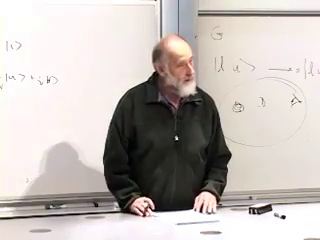
\includegraphics[width=0.66\textwidth]{lecture_07_figure_06.png}
\caption{Концептуальный переход от заданного кета к описанию ансамбля.}
\lectureframe{01:29:43}
\end{figure}

Если состояние \(|i\rangle\) приготовлено с вероятностью \(\rho_i\), то оператор плотности имеет вид
\begin{equation}
\rho=\sum_i\rho_i|i\rangle\langle i|.
\end{equation}
В базисе приготовления
\begin{equation}
\rho=
\begin{pmatrix}
\rho_1&0&0&\cdots\\
0&\rho_2&0&\cdots\\
0&0&\rho_3&\cdots\\
\vdots&\vdots&\vdots&\ddots
\end{pmatrix}.
\end{equation}

\begin{figure}[htbp]
\centering
\includegraphics[width=0.68\textwidth]{lecture_07_figure_09.png}
\caption{Диагональная матрица плотности и условие её нормировки.}
\lectureframe{01:32:12}
\end{figure}

Её собственные значения вещественны и неотрицательны, а нормировка вероятностей принимает вид
\begin{equation}
\operatorname{Tr}\rho=\sum_i\rho_i=1.
\end{equation}

Пусть \(F\) — эрмитова наблюдаемая. Тогда среднее по ансамблю равно
\begin{equation}
\langle F\rangle=\operatorname{Tr}(F\rho).
\end{equation}

\begin{figure}[htbp]
\centering
\includegraphics[width=0.68\textwidth]{lecture_07_figure_10.png}
\caption{Среднее значение, выраженное через след, \(\langle F\rangle=\operatorname{Tr}(F\rho)\).}
\lectureframe{01:35:05}
\end{figure}

Чтобы восстановить обычное взвешенное среднее, вычислим след в базисе, где \(\rho\) диагональна, и вставим разложение единицы:
\begin{align}
\operatorname{Tr}(F\rho)
&=\sum_i\langle i|F\rho|i\rangle\\
&=\sum_{i,j}\langle i|F|j\rangle
               \langle j|\rho|i\rangle\\
&=\sum_i\rho_i\langle i|F|i\rangle.
\end{align}
Таким образом, каждое среднее по чистому состоянию взвешивается вероятностью того, что было приготовлено соответствующее состояние.

След обладает циклическим свойством
\begin{equation}
\operatorname{Tr}(AB)=\operatorname{Tr}(BA),
\end{equation}
даже если \(A\) и \(B\) не коммутируют. Следовательно, \(\operatorname{Tr}(F\rho)=\operatorname{Tr}(\rho F)\).

\section{Квантовая энтропия и отложенный результат}

Энтропия матрицы плотности определяется как
\begin{equation}
S(\rho)=-\operatorname{Tr}(\rho\log\rho).
\end{equation}
Для эрмитова положительного оператора функции, такие как \(\log\rho\), определяются через его собственные значения. Если
\begin{equation}
\rho=\sum_i\rho_i|i\rangle\langle i|,
\end{equation}
то
\begin{equation}
\log\rho=\sum_{\rho_i>0}(\log\rho_i)|i\rangle\langle i|,
\end{equation}
и, следовательно,
\begin{equation}
S(\rho)=-\sum_i\rho_i\log\rho_i.
\end{equation}

\begin{figure}[htbp]
\centering
\includegraphics[width=0.68\textwidth]{lecture_07_figure_11.png}
\caption{Классическая формула энтропии, переписанная в виде \(S=-\operatorname{Tr}(\rho\log\rho)\).}
\lectureframe{01:41:25}
\end{figure}

Известное чистое состояние имеет оператор плотности
\begin{equation}
\rho_\psi=|\psi\rangle\langle\psi|,
\end{equation}
с собственными значениями \(1,0,\ldots\), так что \(S(\rho_\psi)=0\). Это не означает, что для \(|\psi\rangle\) любое измерение имеет определённый результат. Это означает, что о приготовленном состоянии нет никакого дополнительного статистического незнания. На противоположном пределе,
\begin{equation}
\rho=\frac{I}{d}
\qquad\Longrightarrow\qquad
S(\rho)=\log d,
\end{equation}
где \(d=\dim\mathcal H\). Максимально смешанное состояние приписывает одинаковый вес каждому ортогональному направлению.

Теперь мы уже вплотную подошли к связи с запутанностью, но она ещё не проработана. Предположим, что составная система \(AB\) находится в совместном состоянии, а все эксперименты ограничены \(A\). Должен существовать объект, который воспроизводит все средние значения, которые можно получить на \(A\), если \(B\) игнорируется. Этим объектом является матрица плотности для \(A\). Если совместное состояние факторизуется, матрица плотности \(A\) является чистой и имеет нулевую энтропию. Если \(A\) и \(B\) запутаны, то матрица плотности \(A\), вообще говоря, является смешанной и имеет ненулевую энтропию. Построение этой редуцированной матрицы плотности и вычисление её энтропии — задача, отложенная до следующей лекции.
